\documentclass[tikz]{standalone}
\begin{document}

\usetikzlibrary{decorations.pathreplacing}
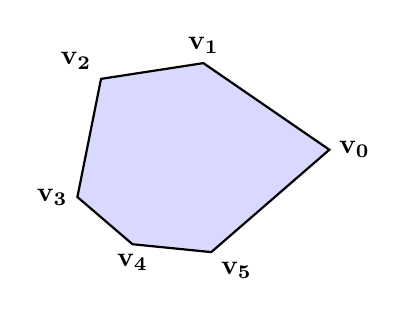
\begin{tikzpicture}


\newcommand{\mvec}[1]{\mathbf{#1}}
\newcommand{\gvec}[1]{\boldsymbol{#1}}

  \definecolor{polcol}{rgb}{0.85,0.85,1.0}

 \coordinate (v0) at (+2.0,+0.5);
 \coordinate (v1) at (+0.4,+1.6);
 \coordinate (v2) at (-0.9,+1.4);
 \coordinate (v3) at (-1.2,-0.1);
 \coordinate (v4) at (-0.5,-0.7);
 \coordinate (v5) at (+0.5,-0.8);

 \coordinate (o) at (+0.05,0.31666);

 % on the opposite side of o.
 \coordinate (r) at (2.35,1.68334);

 \tikzset{
      polstl/.style={thick,fill=polcol},
    }

% 2.35    , 1.68334

 \filldraw[polstl] (v0) -- (v1) -- (v2) -- (v3) --
 (v4) -- (v5) -- cycle;

 \draw (v0) node[right] {$\mvec{v_0}$};
 \draw (v1) node[above] {$\mvec{v_1}$};
 \draw (v2) node[above left] {$\mvec{v_2}$};
 \draw (v3) node[left] {$\mvec{v_3}$};
 \draw (v4) node[below] {$\mvec{v_4}$};
 \draw (v5) node[below right] {$\mvec{v_5}$};
\end{tikzpicture}

\end{document}
